\thispagestyle{empty}
\chapter{The evolutionary forces that shape genomes}
\vspace*{-20pt}
{\hypersetup{linkcolor=GREYDARK}\minitoc}
\label{chap:intro-evol_forces}

In the preceding section, we delved into the fundamental concepts of genomes, gene structure, and expression, which represent the focal points of investigation in my thesis. The current section aims to provide a description of the evolutionary forces shaping genomes and their nucleotide composition over time, based on several reviews. %\citep{crow_perspective_2002, nei_selectionism_2005, keynes_william_2008, nei_neutral_2010, nei_roles_2011, bacaer_wright_2011, abanda_regulation_2012, burkhardt_lamarck_2013, baxter_eb_2017, kovac_lamarck_2019, fairbanks_mendel_2020, berry_mendel_2022, charlesworth_fishers_2022, zhang_masatoshi_2023}. 

We will explore the history of population genetics, investigating the emergence and acceptance of various concepts within the scientific community. Exploring how conceptual ideas and findings that emerge over time provides insight and a better understanding of the evolutionary forces that shape genomes architecture, their impact, and how we estimate them today.

Subsequently, we will describe the mechanisms governing \acrshort{DNA} changes within individual genomes and populations. Our analysis extends to the intricate processes underlying genetic changes, called mutations.

Lastly, we will delve into the dynamics of \acrshort{DNA} variation propagation, specifically the transmission of gene variants, called alleles, within populations. This investigation aims at identifying the primary drivers responsible for the observed evolutionary dynamics, such as the joint product of selection and genetic drift.

\section{Evolution of Evolutionary biology}

I divided the history of evolutionary biology, from its inception to the present day, into four distinct phases spanning the 19th and 21st centuries (\hyperref[fig:chronology_bioevol]{Fig. 2.1}; \citet{riede_why_2010}).

\subsection{Various sub-disciplines (1850-1930)}

Jean Baptiste Lamarck was one of the first to introduce the idea of the evolution of life in his book “Philosophie Zoologique"~\citep{lamarck_philosophie_1809}. Lamarck proposed that individual organisms could modify their organs through use and transmit these changes to their offspring. He illustrated this with the example of giraffes, suggesting that their necks became long because individuals intentionally stretched them to reach leaves. In summary, Lamarck believed that the use of an organ could lead to modifications that could be inherited by the next generation.

Soon after, a young biologist named Charles Darwin set sail on a scientific expedition at the age of 22 aboard the HMS Beagle between 1831 and 1836. During this journey, Darwin observed various species in their natural habitats that eventually led him to publish his renowned book “On the Origin of Species" in 1859, proposing that organisms evolved from a single common ancestor and that these changes were primarily driven by natural selection (see \nameref{selection} section;~\citet{darwin_origin_1859}). According to Darwin, spontaneous morphological or physiological variations arise between offspring, making some individual better adapted to their environment. Such individuals are more likely to survive and transmit their advantageous traits to subsequent generations~\citep{nei_selectionism_2005}.

Contrary to Lamarck, Darwin argued that the elongation of a giraffe's neck was not due to the individual stretching its neck, but rather the result of giraffes with longer necks having a survival advantage over those with shorter necks in reaching food and passing on this trait to future generations through natural selection. Additionally, in 1868, Darwin proposed his theory of heredity through “pangenesis", suggesting that each part of an organism's body emitted small organic particles called gemmules. These gemmules would aggregate in the gonads and contribute heritable information to the gametes~\citep{darwin_variation_1868}. It is now known that this theory was inaccurate, but it is interesting to note that Darwin's pangenesis allowed for the possibility of Lamarckian transmission of acquired characteristics, making him somewhat supportive of Lamarck's ideas while emphasizing the role of natural selection as the main driver of evolutionary changes~\citep{kovac_lamarck_2019}. Currently, the term “Lamarckism" is often used to refer to the inheritance of acquired characteristics, such as epigenetic inheritance, which remains a topic of controversy in modern evolutionary biology~\citep{burkhardt_lamarck_2013}.

During the late 19th and early 20th centuries, significant advances were made not only through observations, but also through the application of rigorous protocols and experiments. Charles Darwin, besides his observations, conducted a series of smaller experiments to investigate how species appeared in different geographic locations. His investigations included studying seed germination conditions and the phenomenon of snails adhering to ducks' feet. However, it was Gregor Johann Mendel, a monk, who introduced the concept of protocols in 1856 by initiating a series of plant hybridization experiments in the monastery gardens. Mendel's goal was to explore how phenotypical traits are inherited across generations. Over a period of seven years, between 1856 and 1863, Mendel cultivated and tested approximately 28,000 plants, with a majority of them being pea plants. Mendel's rigorous plant hybridization experiments and his meticulous observations laid the groundwork for the field of genetics.

Indeed, in 1865, Mendel published a paper in which he proposed that phenotypic traits are passed down to offspring according to the notion of dominant and recessive traits. He also elucidated the phenotypic ratio (9:3:3:1) observed in dihybrid crosses for heterozygous organisms, which is now recognized as the basic law of independent assortment and the law of dominance~\citep{mendel_versuche_1865}. Remarkably, Mendel was familiar with Darwin's work, and historians agree that he accepted Darwin's proposition. In a letter, Mendel even proposed a Darwinian scenario for natural selection, using the same German term for “struggle for existence" as found in his copies of Darwin's books~\citep{fairbanks_mendel_2020, berry_mendel_2022}. 

Mendel's groundbreaking work, however, was not fully appreciated until much later. Indeed, it wasn't until the early 1900s that three biologists, namely Hugo de Vries, Carl Correns, and Erich von Tschermak-Seysenegg, independently rediscovered Mendel's laws, giving due recognition to his significant contributions to the understanding of genetics~\citep{keynes_william_2008}. This era witnessed remarkable progress in comprehending heredity and evolution, mainly due to the pioneering efforts of eminent scientists. Furthermore, Hugo de Vries, through his experimental study of new varieties of evening primrose in his experimental garden, proposed the “macromutation theory", suggesting that spontaneous variations could occur, leading to new traits in organisms~\citep{vries_mutationstheorie_1901}.

Then, in 1909, Thomas Morgan worked on variants of Drosophila, particularly focusing on phenotypic variations in their eyes. Initially skeptical of Mendel's work and Darwin's theory, Morgan's investigations confirmed Mendel's observations in the fruit fly \textit{Drosophila melanogaster}, leading to the publication of his seminal work “The Mechanism of Mendelian Heredity" in 1915~\citep{morgan_mechanism_1915}. Morgan's findings further led him to suggest that natural selection acts as a mechanism to preserve advantageous variations (mutations) while eliminating deleterious ones. However, he argued that the occurrence of advantageous mutations is the primary driver of evolution, meaning that neutral or deleterious ones play a secondary role~\citep{morgan_evolution_1925, allen_thomas_1968}.

Around the same time, R.A. Fisher authored a book, exploring how morphological variations (mutations) can be passed down through generations based on their impact on the ability to produce offspring (fitness) and the number of individuals in the population (population size), using mathematical modeling~\citep{fisher_024_1922, crow_perspective_2002, abanda_regulation_2012, charlesworth_fishers_2022}.

To gain a comprehensive understanding of evolutionary biology, scientists have faced the challenge of reconciling diverse disciplines, such as evolutionary concepts, biological observations, botanical experiments, and population genetics. The integration of these diverse fields was necessary to better understand the complexity of evolutionary processes.


\begin{figure}[H]
    \centering
    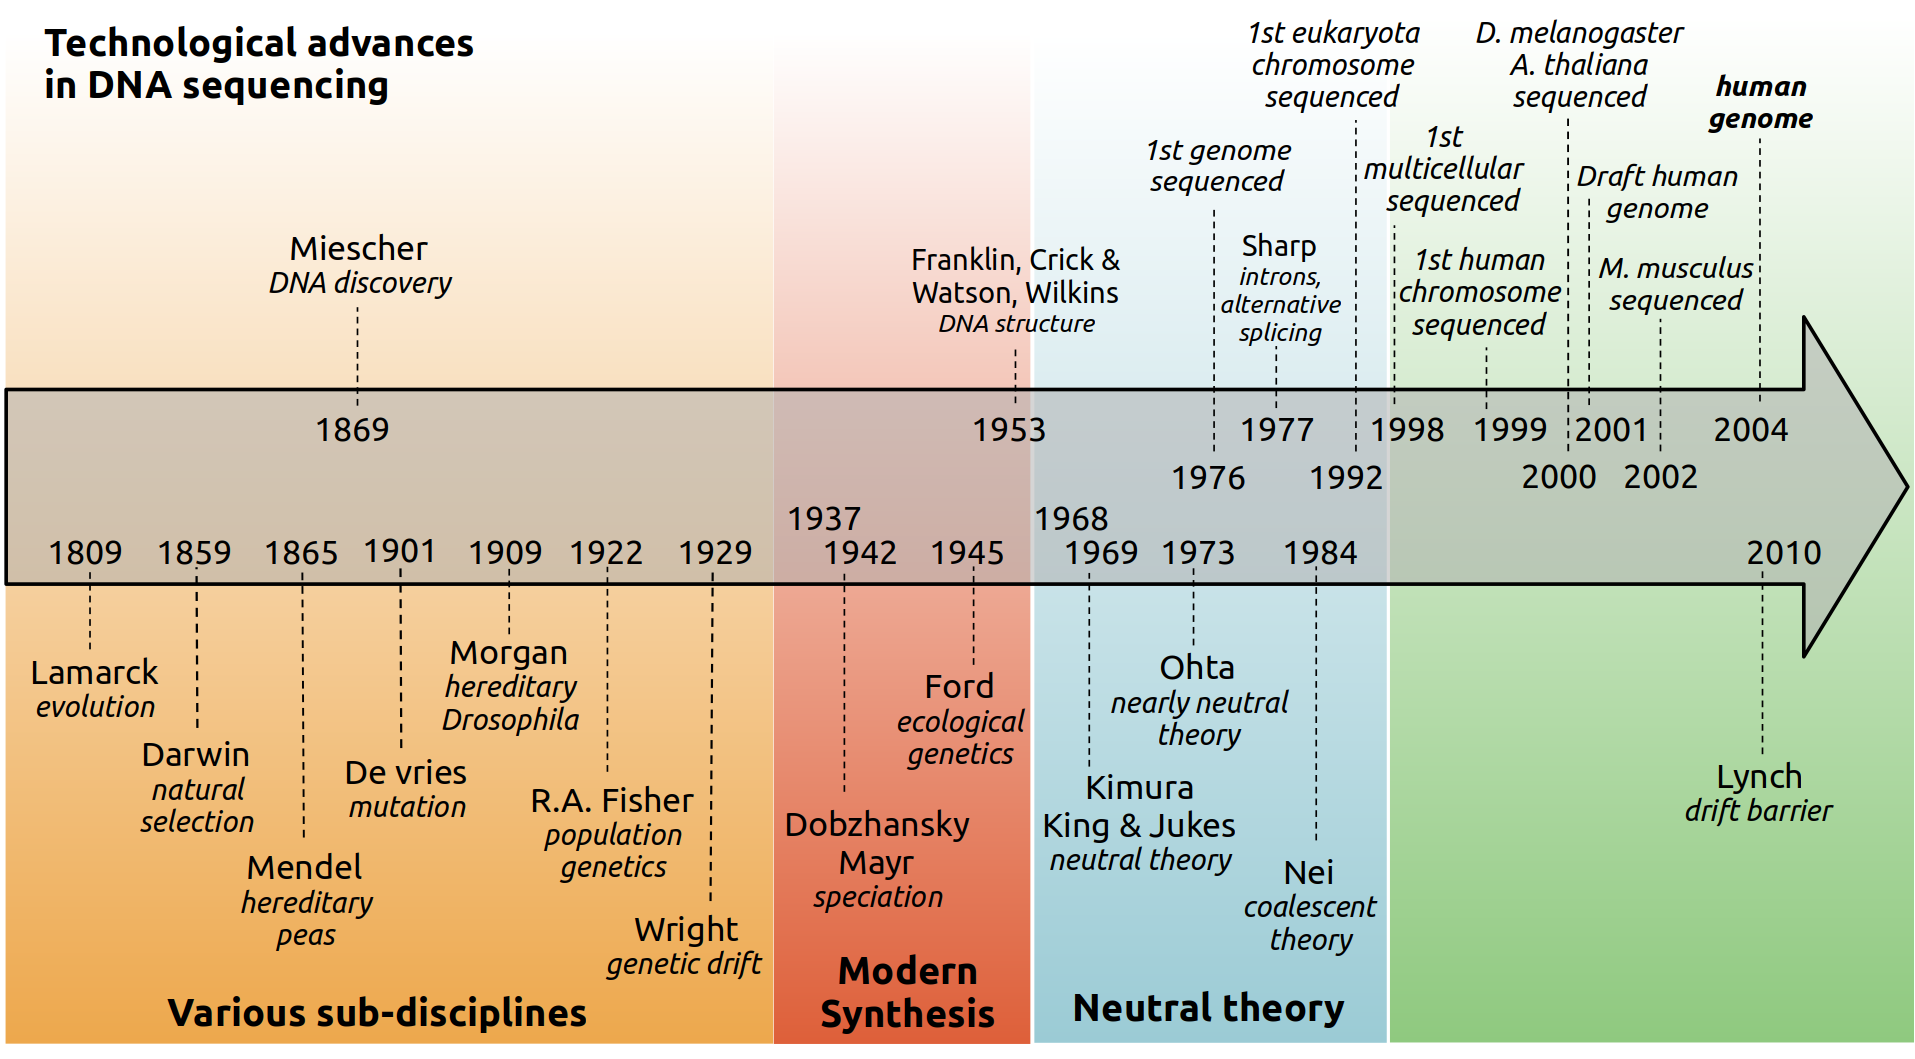
\includegraphics[width=\linewidth]{figures/chronology_bioevol.png}
    \caption[Chronology of Evolutionary biology]{\textbf{Chronology of Evolutionary biology.} Chronology of the different discoveries in evolutionary biology delimiting different periods. Above the timeline are key dates for technological advances associated with \acrshort{DNA} sequencing. Meanwhile, the lower section presents key discoveries in the field of evolutionary biology.}
    \label{fig:chronology_bioevol}
\end{figure}

\subsection{Modern synthesis (1930-1966)}

The “modern synthesis" refers to the formulation of evolutionary theory during the early to mid-20th century, which aimed to reconcile classical Darwinian selection theory with the emerging population-oriented perspective of Mendelian genetics, seeking to elucidate the origin of biological diversity. This period witnessed the confluence of various disciplines, resulting in significant contributions and advancements in evolutionary biology.

Various scientists made valuable contributions to this synthesis. Theodosius Dobzhansky, a postdoctoral researcher in Morgan's fruit fly lab, pioneered the application of genetics to natural populations through experimental studies, primarily focusing on \textit{Drosophila pseudoobscura}. In his seminal book, “Genetics and the Origin of Species" published in 1937, Dobzhansky proposed an explanation for the emergence of new species based on the theoretical developments of natural selection as a genetic process: natural mutations constantly arise within populations~\citep{dobzhansky_genetics_1937, ayala_genetics_1997, barahona_theodosius_2005}. While some mutations can be detrimental under specific conditions, a remarkable portion of these genetic changes have no discernible impact on the organisms' fitness. These neutral mutations persist in different populations and contribute to an unexpectedly vast level of genetic variability, surpassing previous scientific expectations. Dobzhansky's work highlighted the prevalence of neutral mutations in populations. This integration of population genetics with experimental evidence has played a pivotal role in reconciling theoretical concepts with real-world observations.

Fisher, in his seminal work “The Genetical Theory of Natural Selection"~\citep{fisher_genetical_1930, leigh_modern_1999}, demonstrated mathematically how Mendelian genetics could be reconciled with the concept of evolution through natural selection. Also, E.B. Ford, a pioneering experimental naturalist, played a crucial role in the development of ecological genetics as a scientific discipline. By conducting innovative experiments in nature, he aimed to validate the principles of natural selection. Ford's groundbreaking research focused on wild populations of butterflies and moths, and through close collaboration with R.A. Fisher, he successfully confirmed Fisher's predictions~\citep{fisher_spread_1947, ford_butterflies_1945, baxter_eb_2017}.

During this time, Sewall Wright was credited with introducing the term “drift" in his work~\citep{wright_evolution_1929}. Initially, he used it as \textit{“the results of a directed process, selection"} but later clarified its definition as “Random drift"~\citep{wright_random_1970}. The concept of genetic drift acts as a counterbalance to the effect of selection, wherein the chance of a particular variant spreading depends on its selection coefficient and the size of the population ($N$) (see \nameref{geneticdrift} section;~\citet{wright_evolution_1931, wright_sewall_and_others_roles_1932}). The contributions of both Wright and Fisher laid the foundation for the development of population genetics, where mathematical equations were used to establish connections between natural selection and Mendelian genetics.

An intriguing and contentious scientific debate arose between Fisher and Wright. Despite using different methodologies, their theoretical conclusions for a given problem were congruent. Their discrepancies lay in their interpretations rather than in the mathematical aspects. The focal point of the debate revolved around the significance of genetic drift, which Wright referred to as “random sampling" at that time~\citep{wright_fisher_1951}. Ford and Fisher examined color polymorphism frequencies in a population and argued that the population size was too large for these frequency changes to be attributed to drift. Consequently, they suggested that fluctuating selection must be the driving force. As a result, they posited that genetic drift would have minimal impact on phenotypic traits in the vast majority of natural populations~\citep{fisher_sewall_1950, ohara_comparing_2005}, whereas Wright maintained that fluctuations in population size could offer the greatest chance for evolutionary novelty and significantly accelerate evolution~\citep{bacaer_wright_2011}.

\subsection{Neutral and Nearly neutral theory (1966-1990)}

A significant figure in the fields of evolutionary biology and population genetics during the period from 1966 to 1990 was Motoo Kimura. It was during this era that the genetic support, DNA, was initially uncovered. In 1969, Kimura introduced the neutral theory of molecular evolution, which suggests that the majority of evolutionary changes within and between species are primarily driven by random genetic drift of mutant alleles that have no significant impact on an organism's fitness. This theory posits that the vast majority of mutations are not influenced by natural selection. While earlier scientists, such as Fisher, had mathematically derived aspects of neutral mutation theory, they considered it to be rare~\citep{fisher_xviidistribution_1931}. However, Kimura was the first to present a coherent theory of neutral evolution in 1968, which was independently proposed by King and Jukes in 1969, with a focus on differences within species rather than among species~\citep{kimura_evolutionary_1968, king_non-darwinian_1969}.

Kimura and Jukes proposed the non-adaptive theory, suggesting that the majority of mutations are neutral, leading to high substitution rates compared to what one would expect under purifying selective pressures. Therefore, if these modifications persist, it is because they are either neutral or nearly neutral. Over time, as our understanding of genetics advanced, Kimura was able to find evidence supporting his neutral theory of evolution~\citep{kimura_recent_1991}. Notably, he focused on DNA positions that do not affect the translated amino acid due to genetic code redundancy (\gls{synonymous} positions). His observations revealed that these positions exhibit as much variation as expected under the neutral theory, thereby reinforcing the idea proposed by King and Jukes in 1969~\citep{kimura_preponderance_1977}. Additionally, Kimura investigated enzyme (protein) diversity within populations, or polymorphisms, in Drosophila and humans, where multiple forms of the enzyme can coexist, as previously demonstrated by the molecular biologist Richard Lewontin~\citep{lewontin_molecular_1966, harris_enzyme_1966, charlesworth_hubby_2016}. Kimura suggested that most of these forms are selectively neutral, explaining the observed level of heterozygosity through neutral variations.

This gave rise to a long-standing debate between neutralists and selectionists (Neo-Darwinian proponents). While neo-Darwinian scientists firmly believed that species variations are primarily shaped by natural selection, Kimura opposed this view with his neutral theory. Selectionists justified the high genetic diversity within species by claiming that these polymorphisms are maintained by balancing selection, the fact that different alleles of a genes are effectively maintained by natural selection. Whereas neutralists considered that these variations are simply due to neutral changes, that does not necessarily affect the fitness of an individual~\citep{kimura_protein_1971, nei_selectionism_2005, lee_balancing_2021}.

After working and collaborating as a postdoc under Kimura on the neutral theory of evolution, Tomoko Ohta came to the conclusion that the classification of mutations into good, neutral, and harmful was an overly simplistic model insufficient to account for the observed data. Ohta emphasized the significance of nearly neutral mutations, particularly slightly deleterious ones~\citep{ohta_slightly_1973}. The dynamics of nearly neutral mutations closely resemble those of neutral mutations unless the selection coefficient's absolute magnitude exceeds the inverse of the number of individuals (population size). Consequently, the population size can influence the number of mutations considered neutral or deleterious~\citep{ohta_nearly_1992}. 

Another significant contributor to the neutral theory is Masatoshi Nei, who made predictions about the existence of a considerable number of duplicate genes and pseudogenes in organisms based on amino acid \gls{substitution} rates, gene duplication, and gene inactivation~\citep{nei_gene_1969, nei_genetic_1984}. During the 1960s and 1970s, there was considerable controversy surrounding protein evolution mechanisms and the maintenance of protein diversity. Analysess by Nei and his collaborators of alleles frequency distribution and the relationship between average heterozygosity and protein divergence between species supported that a substantial portion of protein polymorphism can be explained by the neutral theory~\citep{nei_neutral_2010, zhang_masatoshi_2023}.

\subsection{Drift barrier hypothesis (2010)}

Following the nearly neutral theory, Michael Lynch formulated the “drift barrier” hypothesis~\citep{lynch_frailty_2007, lynch_evolution_2010}, proposing that the optimization of a trait through natural selection in a specific environment will encounter a theoretical limit. As a trait approaches perfection, the fitness gain of beneficial mutation decreases, and at this barrier, the impact of further beneficial mutations becomes limited in overcoming the influence of random \gls{genetic drift}. Consequently, each species or genome reaches an equilibrium between the effectiveness of natural selection in promoting advantageous traits and the stochastic effects introduced by random \gls{genetic drift}. The equilibrium state of a trait is determined by the interplay of both forces, implying that species with smaller population sizes tend to accumulate a genetic burden and be less optimized compared to species with larger population sizes (\hyperref[fig:drift_selection]{Fig. 2.2}). Therefore, beneficial traits are expected to improve with population size, while deleterious traits should reduce. 
In practical applications, the \gls{effective population size} (\acrshort{Ne}) is employed rather than the total census population size. The \gls{effective population size} pertains to a normalized population with stable spatial distribution, sex ratio, and is a measure of the \gls{genetic drift} intensity as detailed in the subsequent section of this manuscript (see \nameref{geneticdrift} for more details).

\begin{figure}[H]
    \centering
    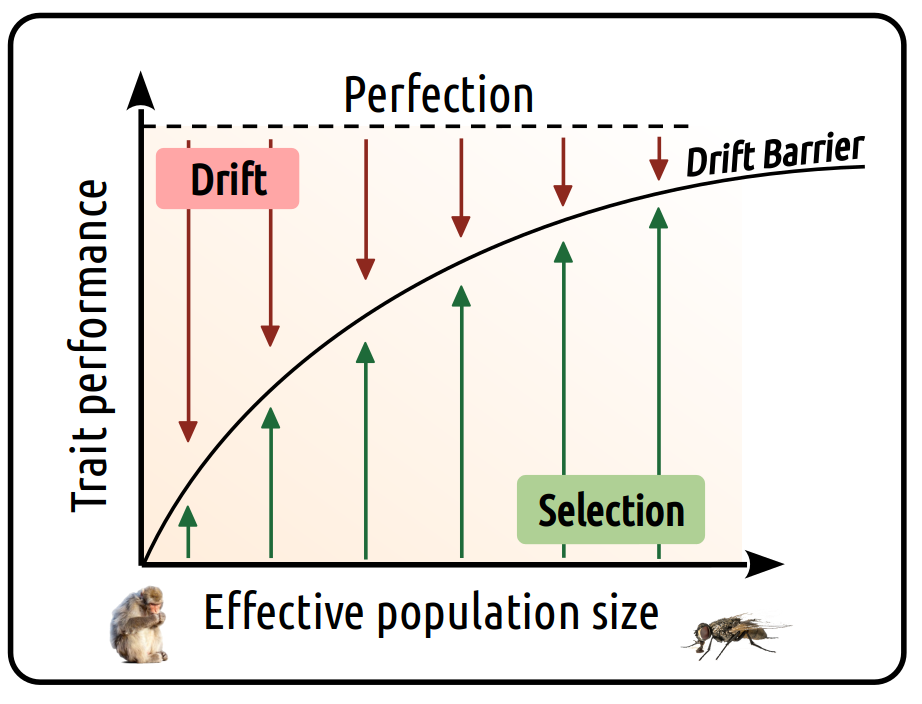
\includegraphics[width=0.6\linewidth]{figures/drift_selection.png}
    \caption[The “drift barrier” hypothesis]{\textbf{The “drift barrier” hypothesis.} Graphic illustrating the “drift barrier” hypothesis according to which the interplay between genetic drift and selection stabilizes a trait performance. Larger population sizes species tend to have better optimized traits compared to smaller population sizes species.}
    \label{fig:drift_selection}
\end{figure}

Lynch presented a compelling argument using mutation rates as an exemple (\textit{i.e.} the number of mutation \textit{per} bp \textit{per} generation) which exhibit considerable variation across species. Selection tends to favor lower mutation rates due to its associated burden of deleterious mutations~\citep{kimura_evolutionary_1967, lynch_cellular_2008}, and since the power of drift is inversely proportional to \acrshort{Ne}, species with larger \acrshort{Ne}~are expected to have lower mutation rates as observed in~\citet{sung_drift-barrier_2012}.

Furthermore, Michael Lynch proposed that variation in the ability to purge slightly deleterious mutations (\textit{i.e.} variation in \acrshort{Ne}) can account for differences in genome architecture among species, such as genome size~\citep{lynch_origins_2003, lefebure_less_2017, merel_relaxed_2024}.

\section{Emergence of new alleles (mutation)}

The mutation theory was first developed by Hugo De Vries in 1901~\citep{vries_mutationstheorie_1901, allen_hugo_1969} when he studied a group of evening primrose, \textit{Oenothera lamarckiana}, where he found that seeds from this plant produced many new varieties in his experimental garden (13 years of experiments). De Vries labeled these sudden and novel variations as “mutations". However, it is important to note a distinction in terminology from De Vries' work: while he broadly characterized any heritable changes in phenotypic traits as mutations, our focus here is on mutations at the DNA level. These modifications are the primary drivers of genetic diversity, ultimately contributing to morphological alterations~\citep{nei_roles_2011}.

Mutations can be classified into four types: base replacements, involving the replacement of one nucleotide with another; small insertions, which involve the addition of one or several nucleotides; small deletions, resulting in the loss of one or several nucleotides; and larger forms of chromosome structural variations (deletions, inversion, translocation or duplication).

If mutations occur within a coding sequence, their impact on the protein product can lead to three different subcategories of mutations: \gls{non-synonymous} mutations, where the modification results in a change in the protein product and may even render the protein non-functional; nonsense mutations, in which the mutation causes premature termination due to the formation of a stop \gls{codon}, mostly leading to an aberrant transcript; and synonymous mutations, occurring when the mutation does not affect the sequence of the protein product~\citep{zia_ranking_2011, potapova_nonsense_2022}.

\subsection{Insertion-deletion}

Small insertion-deletion (\acrshort{Indel}s) are widely distributed throughout the genome and contribute to both intra and inter species divergence~\citep{mcgee_ecological_2020}. These mutations are extensively studied in human genome~\citep{weber_human_2002, bhangale_comprehensive_2005, conrad_high-resolution_2006}. Indels can occur during DNA replication, when the strand that is replicated slips, this can lead to the incorporation or deletion of nucleotides. Also, sequences such as transposable elements possess the particularity to replicate within the genome akin to genome parasites, which induce an insertion at other part of the genome~\citep{cai_transposable_2022, mcclintock_origin_1950}.

A substantial majority of these small \acrshort{Indel}s (96\%) range in length from 1 to 16 \acrshort{bp}, with the largest observed \acrshort{Indel} spanning 55 \acrshort{bp}, as reported by~\citet{mullaney_small_2010}. Notably, \acrshort{Indel}s overlapping coding sequence frequently induce a shift in the reading frame, bearing a high probability of introducing stop \gls{codon}s, thus often resulting in nonsense mutations.


\subsection{Base replacement}

A base replacement occurs when a nucleotide is replaced by another in the genome. Such replacements are categorized as: transitions, \textit{i.e.} involving the exchange between two purines or between two pyrimidines; or transversions, \textit{i.e.} the base replacement between a purine base and a pyrimidine base, or vice versa.

Spontaneous mutations can be caused by external factors such as ionizing radiation, ultraviolet rays, and mutagenic chemicals. These extrinsic agents have the capacity to cause DNA damage, inducing inaccuracies during DNA replication or repair, thus giving rise to mutations~\citep{maki_origins_2002}. Additionally, in the context of dinucleotides CG referred as \gls{CpG} dinucleotides (Cytosyne Phosphate Guanine), following methylation, C-to-U deamination can happen. In mammals the frequent DNA methylation, linked with gene expression regulation, makes \gls{CpG}s highly mutable. This phenomenon explains the lower prevalence of \gls{CpG} dinucleotides in mammals compared to other species~\citep{duncan_mutagenic_1980, brennan_hypermutability_1990}.

Mechanisms exist for the repair of these mutations, involving the comparison of the two DNA strands to identify discrepancies. However, post cell division, the repair machinery becomes challenged, as the newly replicated strands are identical correction mutations is hampered~\citep{gao_mechanisms_2017, cortez_replication-coupled_2019}.

If a base replacement occurs within a coding sequence, it will lead to a modification in the \gls{codon}, yet may not necessarily impact the resulting protein due to the redundancy of the genetic code. It is important to note that not all \gls{non-synonymous} mutations result in an altered protein function. Specifically, if these base replacements occur outside the protein's active site, they might not significantly affect the protein's function, even if the peptide sequence has been altered. An illustrative example is the mutation that converts a leucine (Leu) codon to an isoleucine (Ile) codon ~\citep{sneath_relations_1966, miyata_two_1979, epstein_non-randomness_1967}. Given the chemical similarity between these two amino acids and their potential interchangeability in proteins, such a mutation might not exert a substantial influence on the protein's structure or function, resulting in what is known as a neutral mutation. Likewise, not all synonymous mutations are inherently neutral. Indeed, the composition of \gls{codon}s can influence translation kinetics, thereby impacting the efficiency of protein synthesis and proper folding~\citep{akashi_synonymous_1994, stoletzki_synonymous_2007, drummond_mistranslation-induced_2008, plotkin_synonymous_2011, yang_codon-by-codon_2014, dana_effect_2014, gorochowski_trade-offs_2015, quax_codon_2015, presnyak_codon_2015, wu_translation_2019}.

To calculate the mutation rate \textit{per} base pair \textit{per} generation, one can enumerate the number of replacements occurring within a particular population over a specific generation. This approach facilitates the assessment of the frequency and pace at which new \gls{allele}s can be introduced into a population, consequently contributing to genetic diversity. Mutation rates exhibit significant variation across taxonomic groups and within different genomic regions of a single organism, averaging around 12 x $10^{-9}$ mutation \textit{per} \acrshort{bp} \textit{per} generation in mammalian genomes~\citep{kumar_mutation_2002, lynch_evolution_2010, bergeron_evolution_2023}.

Germ-line mutations arise within gametes or cells that ultimately give rise to gametes. In contrast to somatic mutations, germ-line mutations are heritable and passed down to subsequent generations. Consequently, these mutations contribute to form different version of genes (\gls{allele}s), and are present in all cell types of future organisms, thus have the potential to propagate within a population.

\section{The fate of new alleles}

Alleles in a population are carried by individual genomes and propagate through generations at varying frequency, influenced by diverse forces: selection, \gls{genetic drift} and \gls{biased gene conversion}. A new \gls{allele} within a population reaches fixation when possessed by all individuals, this mutation is then called a \gls{substitution}.


\subsection{Selection}
\label{selection}

The concept of natural selection, introduced by Darwin in is seminal work, underscores the process by which species evolve and adapt. This evolution involves the accumulation of mutations that enhance individual fitness ($w$). The fitness of a genotype or \gls{phenotype} is gauged by its ability to produce offspring. This estimation requires to evaluate the reproductive rate, defined as the average number of offspring produced \textit{per} individual, and the survival rate, which represents the percentage of born individuals that reach reproductive maturity. Consequently, for each genotype, the product of the reproductive rate and survival rate is calculated. The relative fitness of each genotype is derived from this product relative to a reference genotype. Fitness values are $\geq 0$, with 0 signifying that there is no viable descendant.

Expressed as the selection coefficient (\acrshort{s}), the relationship between fitness and selection is given by $\acrshort{s} = w - 1$, a measure of the relative strength of selection acting against a genotype. If \acrshort{s} assumes a negative value, the allele is deemed deleterious and subjected to counter-selection (or purifying selection). Conversely, a positive \acrshort{s} indicates a beneficial \gls{allele}~\citep{redei_selection_2008, coop_population_2020, akashi_within-_1999}.

The force of natural selection stands as a pivotal determinant in the destiny of novel \gls{allele}s within populations. It drives the survival and reproductive success of individuals harboring advantageous \gls{allele}s, thus causing a progressive increase in their prevalence over successive generations. Conversely, \gls{allele}s that are detrimental to survival or reproductive fitness are either purged or maintained at reduced frequencies. 

The effect of counter-selection seems to be amplified in highly expressed genes. Indeed, those genes accumulate \gls{non-synonymous} substitutions, weakly deleterious, at a slower rate than less expressed genes~\citep{duret_determinants_2000, rocha_analysis_2004, pagan_level_2012, brion_evolution_2015} and are more conserved across species~\citep{pal_highly_2001, geiler-samerotte_misfolded_2011, zhang_determinants_2015}. One hypothesis is that misfolded proteins are toxic in cells and selection act to diminish this toxicity~\citep{yang_protein_2012, park_differential_2013, wu_expression_2022, trucchi_gene_2023}. An other hypothesis is based on the fitness cost of deleterious mutations linked with the unnecessary mobilization of metabolic resources and cellular machinery. This fitness cost is more important in highly expressed genes that solicit a lot of resources compared to lowly expressed genes. Consequently, these highly expressed genes tend to be subject to more intense purifying selection, resulting in a more pronounced elimination of deleterious alleles compared to genes with lower expression levels~\citep{saudemont_fitness_2017, nabholz_high_2012}.


\subsection{Genetic drift}
\label{geneticdrift}

As previously mentioned, \gls{genetic drift}, a concept introduced by Wright, refers to stochastic fluctuations in allele frequencies within a population across successive generations. 

These fluctuations arise due to the inherently random sampling of individuals that reproduce and pass on their alleles to subsequent generations. Notably, the impact of \gls{genetic drift} is more pronounced in populations of smaller size, where random variations exert a more substantial influence. The intensity of random \gls{genetic drift} is measured through the concept of the \gls{effective population size} (\acrshort{Ne}). This parameter represents the hypothetical number of individuals within a Hardy-Weinberg population that would yield equivalent patterns of random fluctuations at neutral sites~\citep{husemann_effective_2016, wang_prediction_2016}. In a Hardy-Weinberg population, mating occurs randomly (panmixia), as do encounters between gametes (pangamy). Generations do not overlap, implying that individuals from distinct generations cannot reproduce together. Furthermore, no natural selection, mutation, or migration factors are at play within this context~\citep{hardy_course_1908, wright_evolution_1931, stern_hardy-weinberg_1943, felsenstein_inbreeding_1971, edwards_g_2008}.

\acrshort{Ne}~intervenes in population genetic equations, where the rate of fixation (\acrshort{K}) for newly introduced allele within a \gls{diploïd} population of \acrshort{Ne}~individuals (\textit{i.e.} allele frequency $p=\frac{1}{2\acrshort{Ne}}$) is given by: the number of new mutations in each generation multiplied by the probability of reaching fixation ($P^F$).
\[\acrshort{K} = 2\acrshort{Ne}~\acrshort{mu}~P^F = 2\acrshort{Ne}~\acrshort{mu}~\frac{1 - e^{-4\acrshort{Ne}\acrshort{s} p}}{1 - e^{-4\acrshort{Ne}\acrshort{s}}} = 2\acrshort{Ne}~\acrshort{mu}~\frac{1 - e^{-2s}}{1 - e^{-4\acrshort{Ne}\acrshort{s}}}\]
where \acrshort{s} represents the selection coefficient of the allele and \acrshort{mu} the mutation rate \textit{per} base pair \textit{per} generation.

For neutral alleles where $s\rightarrow 0$, then $\acrshort{K} = \acrshort{mu}$.

Thus, for small selection coefficients, when \acrshort{Ne}~decreases \acrshort{K} approaches \acrshort{mu} , and alleles behave as if they are effectively neutral (\hyperref[fig:Mutationrate]{Fig. 2.3}).

\begin{figure}[H]
    \centering
    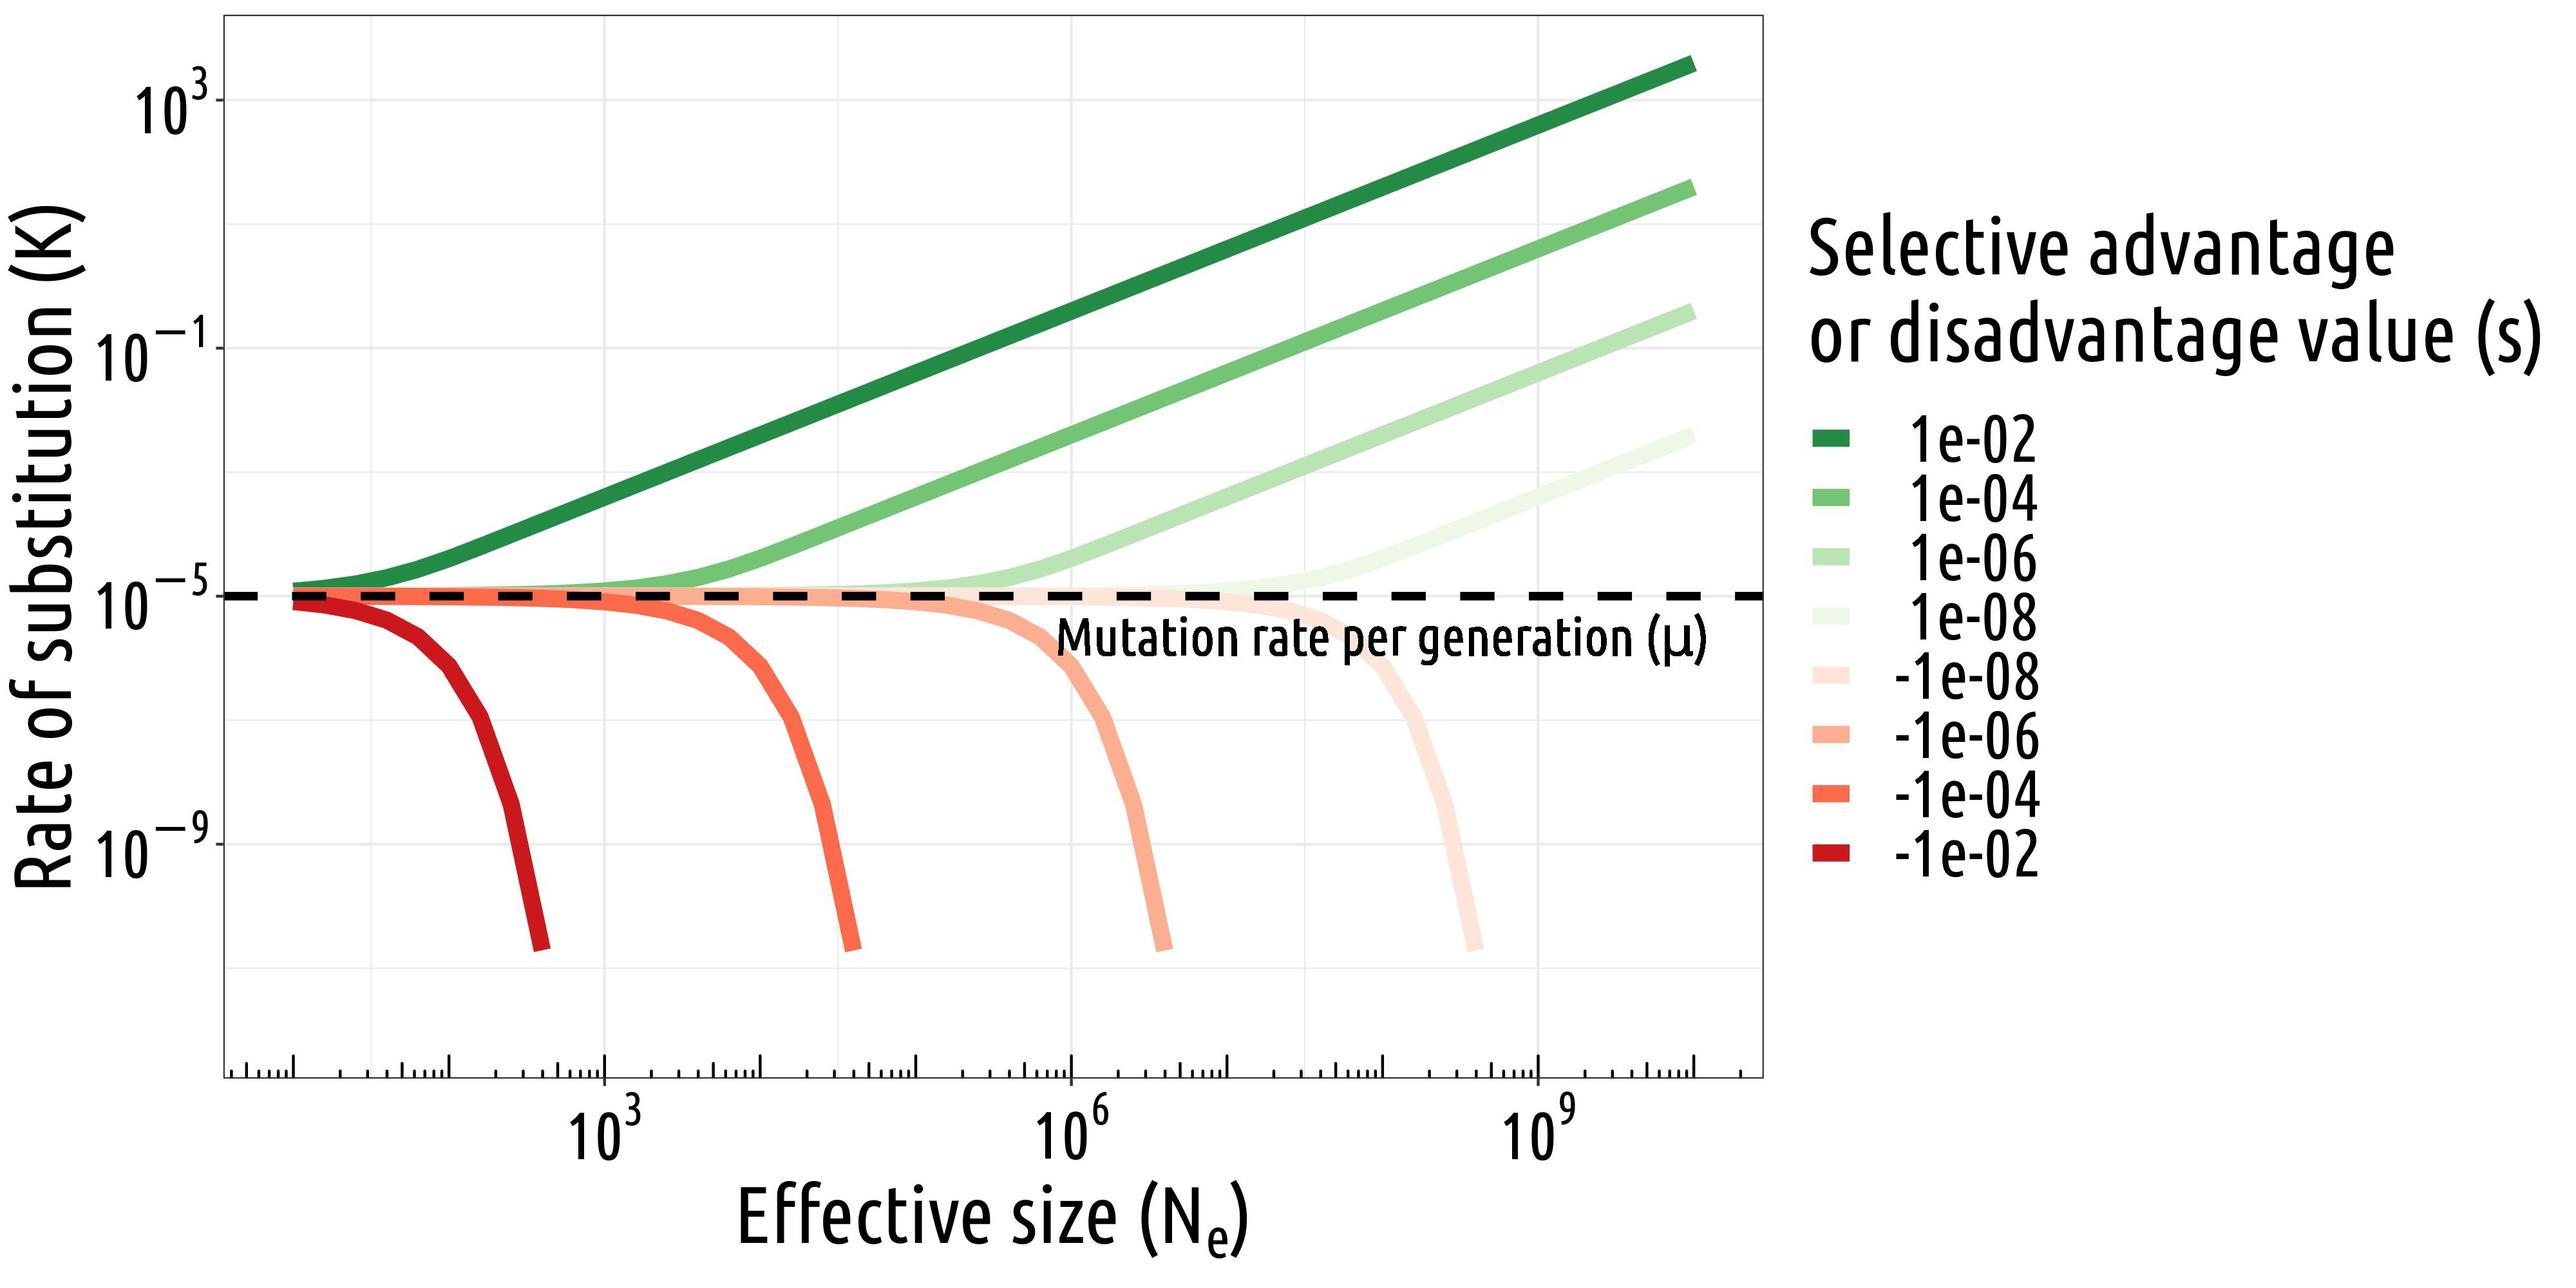
\includegraphics[width=\linewidth]{figures/Mutation rate.png}
    \caption[Substitution rate for slightly deleterious and advantageous alleles]{\textbf{Substitution rate for slightly deleterious and advantageous alleles.} In this simulation, based on equations by~\citet{lynch_origins_2007} we observe that for alleles with a slight selection coefficient ($|s| \ll 1$) as the product of \gls{effective population size} (\acrshort{Ne}) and selection coefficient (\acrshort{s}) decreases, the fixation rate (\acrshort{K} of a particular allele converges towards the neutral rate; \citet{lynch_origins_2007}).}
    \label{fig:Mutationrate}
\end{figure}

In fact, the parameter that matters in determining the ability of selection to promote beneficial mutations or eliminate deleterious mutations is the intensity of selection (\acrshort{s}) relative to the power of random genetic drift (\acrshort{Ne}), called the population-scaled selection coefficient $\acrshort{S} = |4\acrshort{Ne}\acrshort{s}|$ (\hyperref[fig:popscaled]{Fig. 2.4}). If $\acrshort{S} \gg 1$ variations in \acrshort{Ne}~won't affect the fixation probability and selection will be the main force determining the fate of alleles. If the selection coefficient is sufficiently weak relative to drift ($\acrshort{S} \ll 1 $), alleles behave as if they are effectively neutral leaving no grounds for selection. Between both extremes, changes in \acrshort{Ne}~will affect the rate of \gls{substitution}s.

In consequences random genetic drift impact the efficiency of selection in promoting slightly advantageous alleles while suppressing slightly deleterious ones within populations (\hyperref[fig:geneticdrift]{Fig. 2.5}). In low \gls{effective population size}, slightly deleterious alleles can reach fixation due to the strong stochasticity of genetic drift hindering the effect of purifying selection. This led Lynch to propose the “drift barrier” hypothesis where drift limit the genome optimization by overwhelming the selection~\citep{lynch_frailty_2007, lynch_evolution_2010} (\hyperref[fig:drift_selection]{Fig. 2.2}).

\acrshort{Ne}~is generally lower than the census population size (\acrshort{N})~\citep{palstra_genetic_2008, palstra_effectivecensus_2012}. Indeed, variations in population size, difference in sex ratio, and spatial distribution are factors contributing to increase the random drift compare to a Hardy-Weinberg population of the same size~\citep{waples_effective_2002, waples_life-history_2016}. Thus, \acrshort{Ne}~cannot be estimated by simply counting the number of individuals in a population.

\begin{figure}[H]
    \centering
    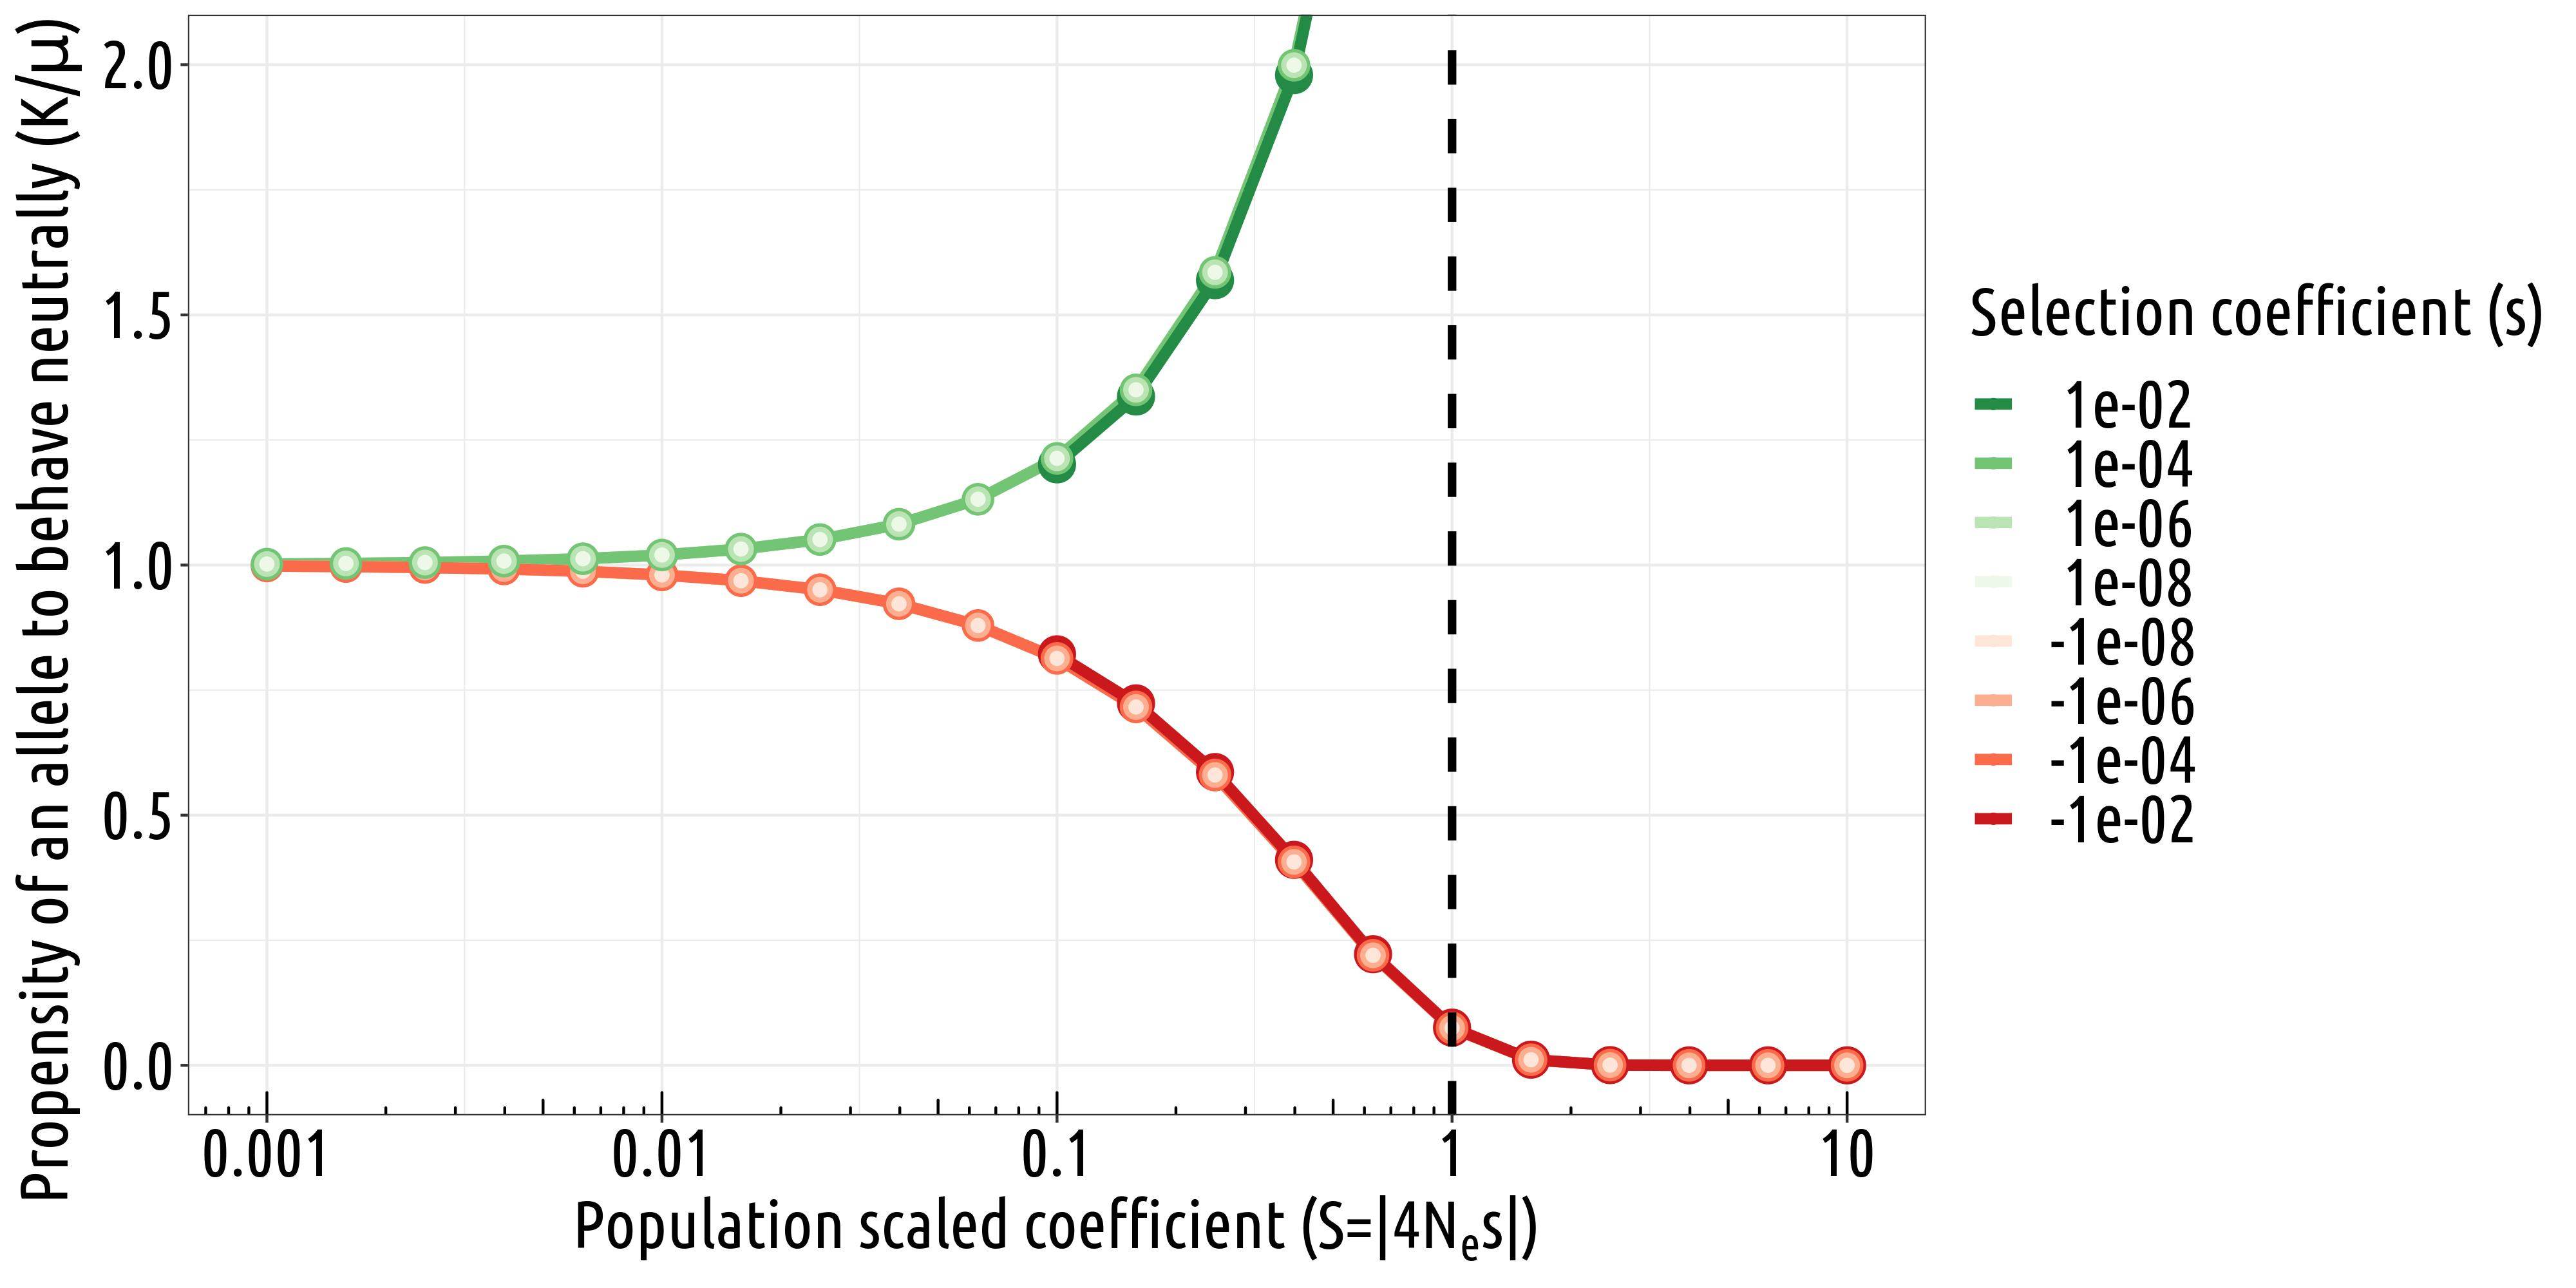
\includegraphics[width=\linewidth]{figures/pop scaled coefficient.png}
        \caption[Population-scaled selection coefficient impact on allele behavior]{\textbf{Population-scaled selection coefficient impact on allele behavior.} Relation between the population-scaled selection coefficient $\acrshort{S} = |4\acrshort{Ne}\acrshort{s}|$ and the propensity of an allele to be neutral, the ratio of \acrshort{K} the \gls{substitution} rate, and the mutation rate \textit{per} base pair \textit{per} generation \acrshort{mu}.}
    \label{fig:popscaled}
\end{figure}


To estimate \acrshort{Ne}~one can directly measure the intensity of drift by quantifying the allele frequency variations through generations at neutral sites. Because in nature this approach needs a lot of resource other estimates have been proposed from population genetic equations. One such is the genetic diversity. At mutation-drift equilibrium the \gls{effective population size} (\acrshort{Ne}) is directly measured by the degree of genetic diversity (average nucleotide heterozygosity at synonymous sites, \acrshort{piS}) within a \gls{diploïd} population expected to be equal to $\approx4\acrshort{Ne} \acrshort{mu}$, \acrshort{mu} being the mutation rate \textit{per} base pair \textit{per} generation. Using this equation, estimates of \gls{effective population size} have been calculated by estimating \acrshort{piS} and \acrshort{mu} with base-substitutional mutation rate/site/cell division in several species~\citep{sung_drift-barrier_2012, lynch_divergence_2023}. With this method, humans have been shown to have a relatively low \acrshort{Ne}$\approx10^4$, compared to \textit{Carnorhabditis} with $10^7$ and Eubacteria reaching $10^8$. 

Also, random linkage disequilibrium, which measures the dependence between two neutral alleles at different loci, is theoretically associated to \acrshort{Ne}~and can be use as an estimator~\citep{waples_practical_2024}. Indeed population recombination rate depends on drift intensity as $\rho = 4\acrshort{Ne}r$, where $r$ is the \textit{per}-generation recombination rate~\citep{waples_linkage_2010}.

\begin{figure}[H]
    \centering
    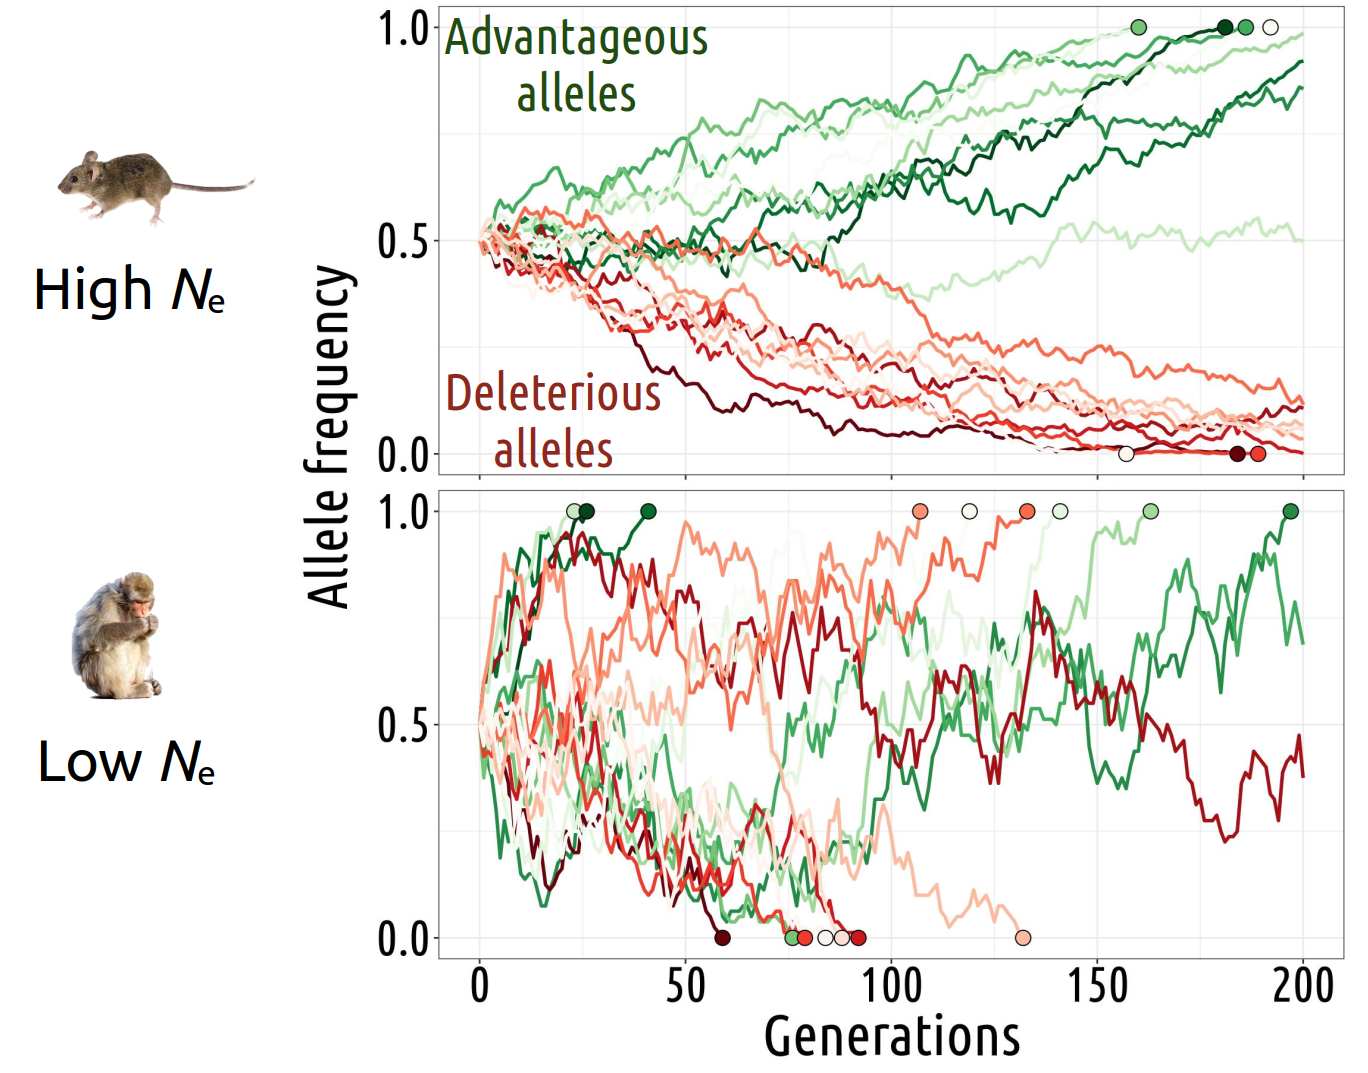
\includegraphics[width=0.7\linewidth]{figures/genetic_drift.png}
    \caption[Genetic drift and its impact on allele fixations]{\textbf{Genetic drift and its impact on allele fixations.} Selection tends to promote advantageous alleles while suppressing deleterious ones. But the efficacy of this evolutionary force diminishes with increasing genetic drift intensity, associated with a reduced \gls{effective population size}. The presented simulations illustrate the variations in frequencies of slightly advantageous (green curves) or deleterious alleles (red curves) across generations, comparing populations with a high \gls{effective population size} (top) to those with a low \gls{effective population size} (bottom).}
    \label{fig:geneticdrift}
\end{figure}


Genetic diversity and population recombination rate are two measures of short time scale \acrshort{Ne}~(short-term \acrshort{Ne}), which may not reflect the \acrshort{Ne}~that affected the genome evolution on large time scale (long-term \acrshort{Ne}). An additional means of approximating \acrshort{Ne}~involves the assessment of the magnitude of purifying selection acting on protein sequences, as indicated by the ratio ${dN}/{dS}$~\citep{kryazhimskiy_population_2008}.
The underlying hypothesis is that the rate of synonymous substitutions ($dS$) quantifies the rate of neutral allele substitutions, while the rate of \gls{non-synonymous} \gls{substitution}s ($dN$) reflects the rate of deleterious allele substitutions (\hyperref[fig:dnds]{Fig. 2.6}). The ratio \dnds represents the efficacy of selection in suppressing deleterious alleles relative to the influence of genetic drift.

Indeed as mentioned earlier, the probability of fixation for a specific allele with a frequency \( p \) within a \gls{diploïd} population of \acrshort{Ne}~individuals is given by
\[ P^F(p) = \frac{1 - e^{-4\acrshort{Ne}\acrshort{s} p}}{1 - e^{-4\acrshort{Ne}\acrshort{s}}} \]

In the case of a \gls{diploïd} species, a newly introduced allele is expected to have a frequency $p = \frac{1}{2\acrshort{Ne}}$, leading to a simplified equation:
\[ P^F(\frac{1}{2\acrshort{Ne}}) = \frac{1 - e^{-2s}}{1 - e^{-4\acrshort{Ne}\acrshort{s}}} \]

For small \acrshort{s} values ($\acrshort{s} \ll 1$), further simplification yields
\[ P^F\left(\frac{1}{2\acrshort{Ne}}\right) \approx \frac{2s}{1 - e^{-4\acrshort{Ne}\acrshort{s}}} \]

The following equations describe the change in the number of \gls{synonymous} ($dS$) and \gls{non-synonymous} (\gls{dN}) mutations over generations:
\[dN = \acrshort{mu} \cdot \text{generations} \cdot P^F_{\text{non-synonymous}}\]
\[dS = \acrshort{mu} \cdot \text{generations} \cdot P^F_{\text{synonymous}}\]

where \( P^F_{\text{synonymous}} \) indicates fixation probability of nearly neutral alleles because \gls{synonymous} substitutions $s \rightarrow 0$, hence $4\acrshort{Ne}\acrshort{s} \rightarrow 0$.

Thus leading to the simplification \( P^F_{\text{synonymous}} = \frac{2\acrshort{s}}{4\acrshort{Ne}\acrshort{s}} = \frac{1}{2\acrshort{Ne}} \)~\citep{kimura_probability_1962}, the case where allele behave as neutral.

For \gls{non-synonymous} substitutions:
\[P^F_{\text{non-synonymous}} \approx \frac{2\acrshort{s}_{\text{non-synonymous}}}{1 - e^{-4\acrshort{Ne}\acrshort{s}_{\text{non-synonymous}}}}\]


The ratio ${dN}/{dS}$ becomes:
\[\frac{dN}{dS} \approx \frac{4\acrshort{Ne}\acrshort{s}_{\text{non-synonymous}}}{1 - e^{-4\acrshort{Ne}\acrshort{s}_{\text{non-synonymous}}}}\]

${dN}/{dS}$ appears as a function of 4\acrshort{Ne}\acrshort{s}~\citep{nielsen_estimating_2003}, and if we assumed \gls{non-synonymous} \gls{substitution} mostly deleterious because of its impact on protein sequences: $\acrshort{s}_{\text{non-synonymous}}< 0$ stable between species, ${dN}/{dS}$ is negatively correlated with \acrshort{Ne}, provided it is in the range where the population-scaled selection coefficient allows it.

The ${dN}/{dS}$ ratio serves as a valuable tool for comparing selective pressures among genes. For example, highly expressed genes tend to have low ${dN}/{dS}$ values, indicating greater constraint, in contrast to genes with lower expression levels~\citep{duret_determinants_2000, rocha_analysis_2004, pagan_level_2012, brion_evolution_2015}.

\begin{figure}[H]
    \centering
    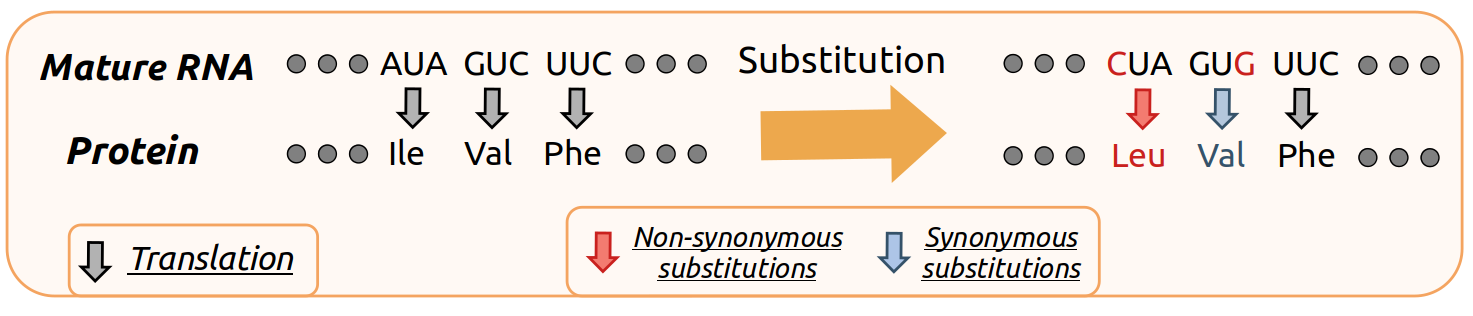
\includegraphics[width=\linewidth]{figures/dnds.png}
    \caption[Non-synonymous and synonymous substitutions]{\textbf{Non-synonymous and synonymous substitutions.} Example of one \gls{non-synonymous} substitution (red) and one \gls{synonymous} substitution (blue) in a partial sequence of three \gls{codon}s. For the \gls{non-synonymous} substitution the isoleucine amino acid is replaced by leucine due to a substitution from adenine to cytosine at the first position of the \gls{codon}. For the \gls{synonymous} substitution the cytosine at the third position is replaced by a guanine which does not change the translated amino acid.}
    \label{fig:dnds}
\end{figure}

Also, various proxies can be employed to examine the relative fluctuations in \gls{effective population size} (\acrshort{Ne}). One such factor is the examination of life history traits such as longevity, body weight, and body length. This is based on the concept that larger organisms tend to have a reduced number of individuals within their ecological niche, thus impacting the overall population size. And if other parameters such as sex ratio, reproductive mode, spatial distributions are not altered, life history traits variations are expected to be linked to \acrshort{Ne}~\citep{waples_life-history_2016, figuet_life_2016, galtier_adaptive_2016, weyna_relaxation_2020}.

Furthermore, the reproductive system contributes to altering \gls{effective population size}. For instance, in eusocial species, most individuals are sterile, and only a limited number of female (queens) and males engages in reproduction and transmits their genetic heritage. Consequently, this process reduces the \gls{effective population size} and subsequently intensifies genetic drift, especially when compared to an equivalent number of individuals within solitary species~\citep{romiguier_population_2014}.

\subsection{Biased gene conversion}

The last evolutionary force developed in this section is the \gls{biased gene conversion}. During meiosis, a \gls{diploïd} cell, characterized by the presence of two homologous chromosomes, undergoes division to produce haploid cells. The pairing of these chromosomes is called genetic recombination, by which genetic exchanges occur between the homologous chromosomes, significantly contributing to the maintenance of genetic diversity within populations. This processes was unveiled by Thomas Morgan's work, but was previously observed in Mendel's plant hybridization.

During recombination, chromosomes harbor a heteroduplex region, wherein the two \acrshort{DNA} strands do not possess identical sequences, because they originate from each homologous chromosome. Repair mechanisms are invoked to ensure nucleotide homogeneity on both DNA strands. In many metazoans, this repair process exhibits a noteworthy preference for guanine-cytosine (GC) content, as documented by previous studies~\citep{duret_impact_2008, duret_biased_2009, romiguier_contrasting_2010}. This preference for repairing towards GC, when faced with the choice between adenine-thymine (AT) or GC, subsequently leads to an asymmetrical propagation of GC alleles, thereby impacting the distribution of genetic variants. This process, known as GC-\gls{biased gene conversion} (\acrshort{gBGC}), is an evolutionary force similar to selection in the sense that it promotes GC alleles over AT alleles. However, this phenomenon of GC-\gls{biased gene conversion} is not universally observed across species~\citep{galtier_fine-scale_2021, mugal_systematic_2021}. Thus, the GC landscape of genomes is highly affected by \acrshort{gBGC} in species where this process is observed. Which can ultimately affect the composition of the coding sequences. Furthermore, this force does not necessarily tend to increase the fitness of individuals, and can even go against it.